\chapter{Experimental Motivation}
\label{ch:experiment}

\section{Introduction}
Can the supercurrent be monitored in a bilayer graphene (BLG) sample? The experimental work underpinning this thesis concerns itself with this question. In a conventional tunnel barrier, the supercurrent can only be tuned when the sample geometry or the environment temperature is changed. Moreover, the tunnel barrier should not exceed a certain width in order to make the supercurrent observable. The central idea of the particular set-up presented here is to create a weak link in the form of a quantum point contact (QPC). A weak link is a conductive material in which superconductivity can be induced because of the superconducting proximity effect \cite{Likharev1979}. The key achievement of this work is showing that with this QPC geometry, the supercurrent can be controlled both in its amplitude as well as in the spatial distribution within the set-up, which has not been observed so far.
\begin{figure}[h]
\centering
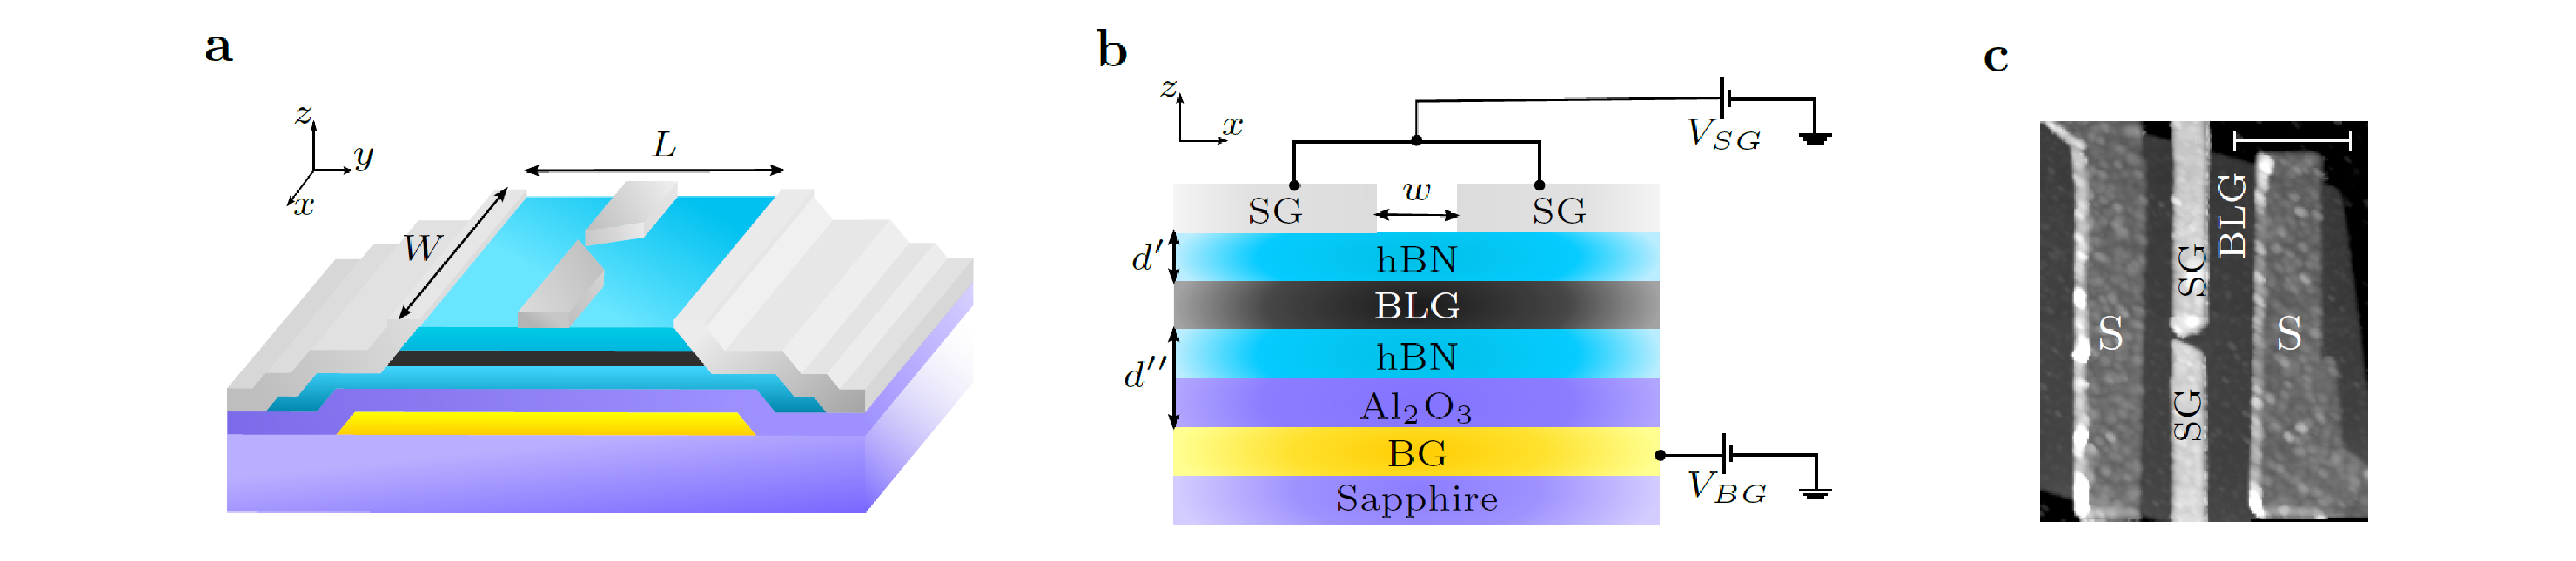
\includegraphics[width=\textwidth]{figure/experiment/setup}
\caption{A schematic of the device. The top view \textbf{a} displays the two fingers of the QPC topgate in the middle of the device. The cross-sectional schematic \textbf{b} shows the superconducting material $\text{Al}_2\text{O}_3$ lying on top of the back gate. The BLG is encapsulated between two layers of hBN. The split width $w$ is the width between the two fingers of the QPC gate. \textbf{c} shows an image of the device, with the scale on the upper right corresponding to $1\ \mu m$.   }\label{fig:setup}
\end{figure}
Figure \ref{fig:setup} shows a schematic of the set-up. The BLG layer (black) is of width $W$ and a length $L$. It is encapsulated between two layers of hexagonal boron nitride (hBN, blue) and lies on top of a back-gate. A top-gate with a split of width $w$ in the middle, as depicted in see figure \ref{fig:setup} b, covers the the heterostructure. This device layout enables tuning the back-gate potential $V_{BG}$ independently from the top-gate or split-gate potential $V_{SG}$.

By gating the material with $V_{BG}$, an overall potential is applied at the whole region, lifting the Fermi energy $E_F$ of the system. At the same time, the region that is covered with the top gate is gated locally by the split-gate potential, while creating a displacement field along the sample. The displacement field breaks the symmetry of the BLG, and the two layers are at different energy levels. As as result, a gap in the BLG spectrum is opened \cite{McCann2006}. 

\section{Normal State Analysis}
\begin{figure}
\centering
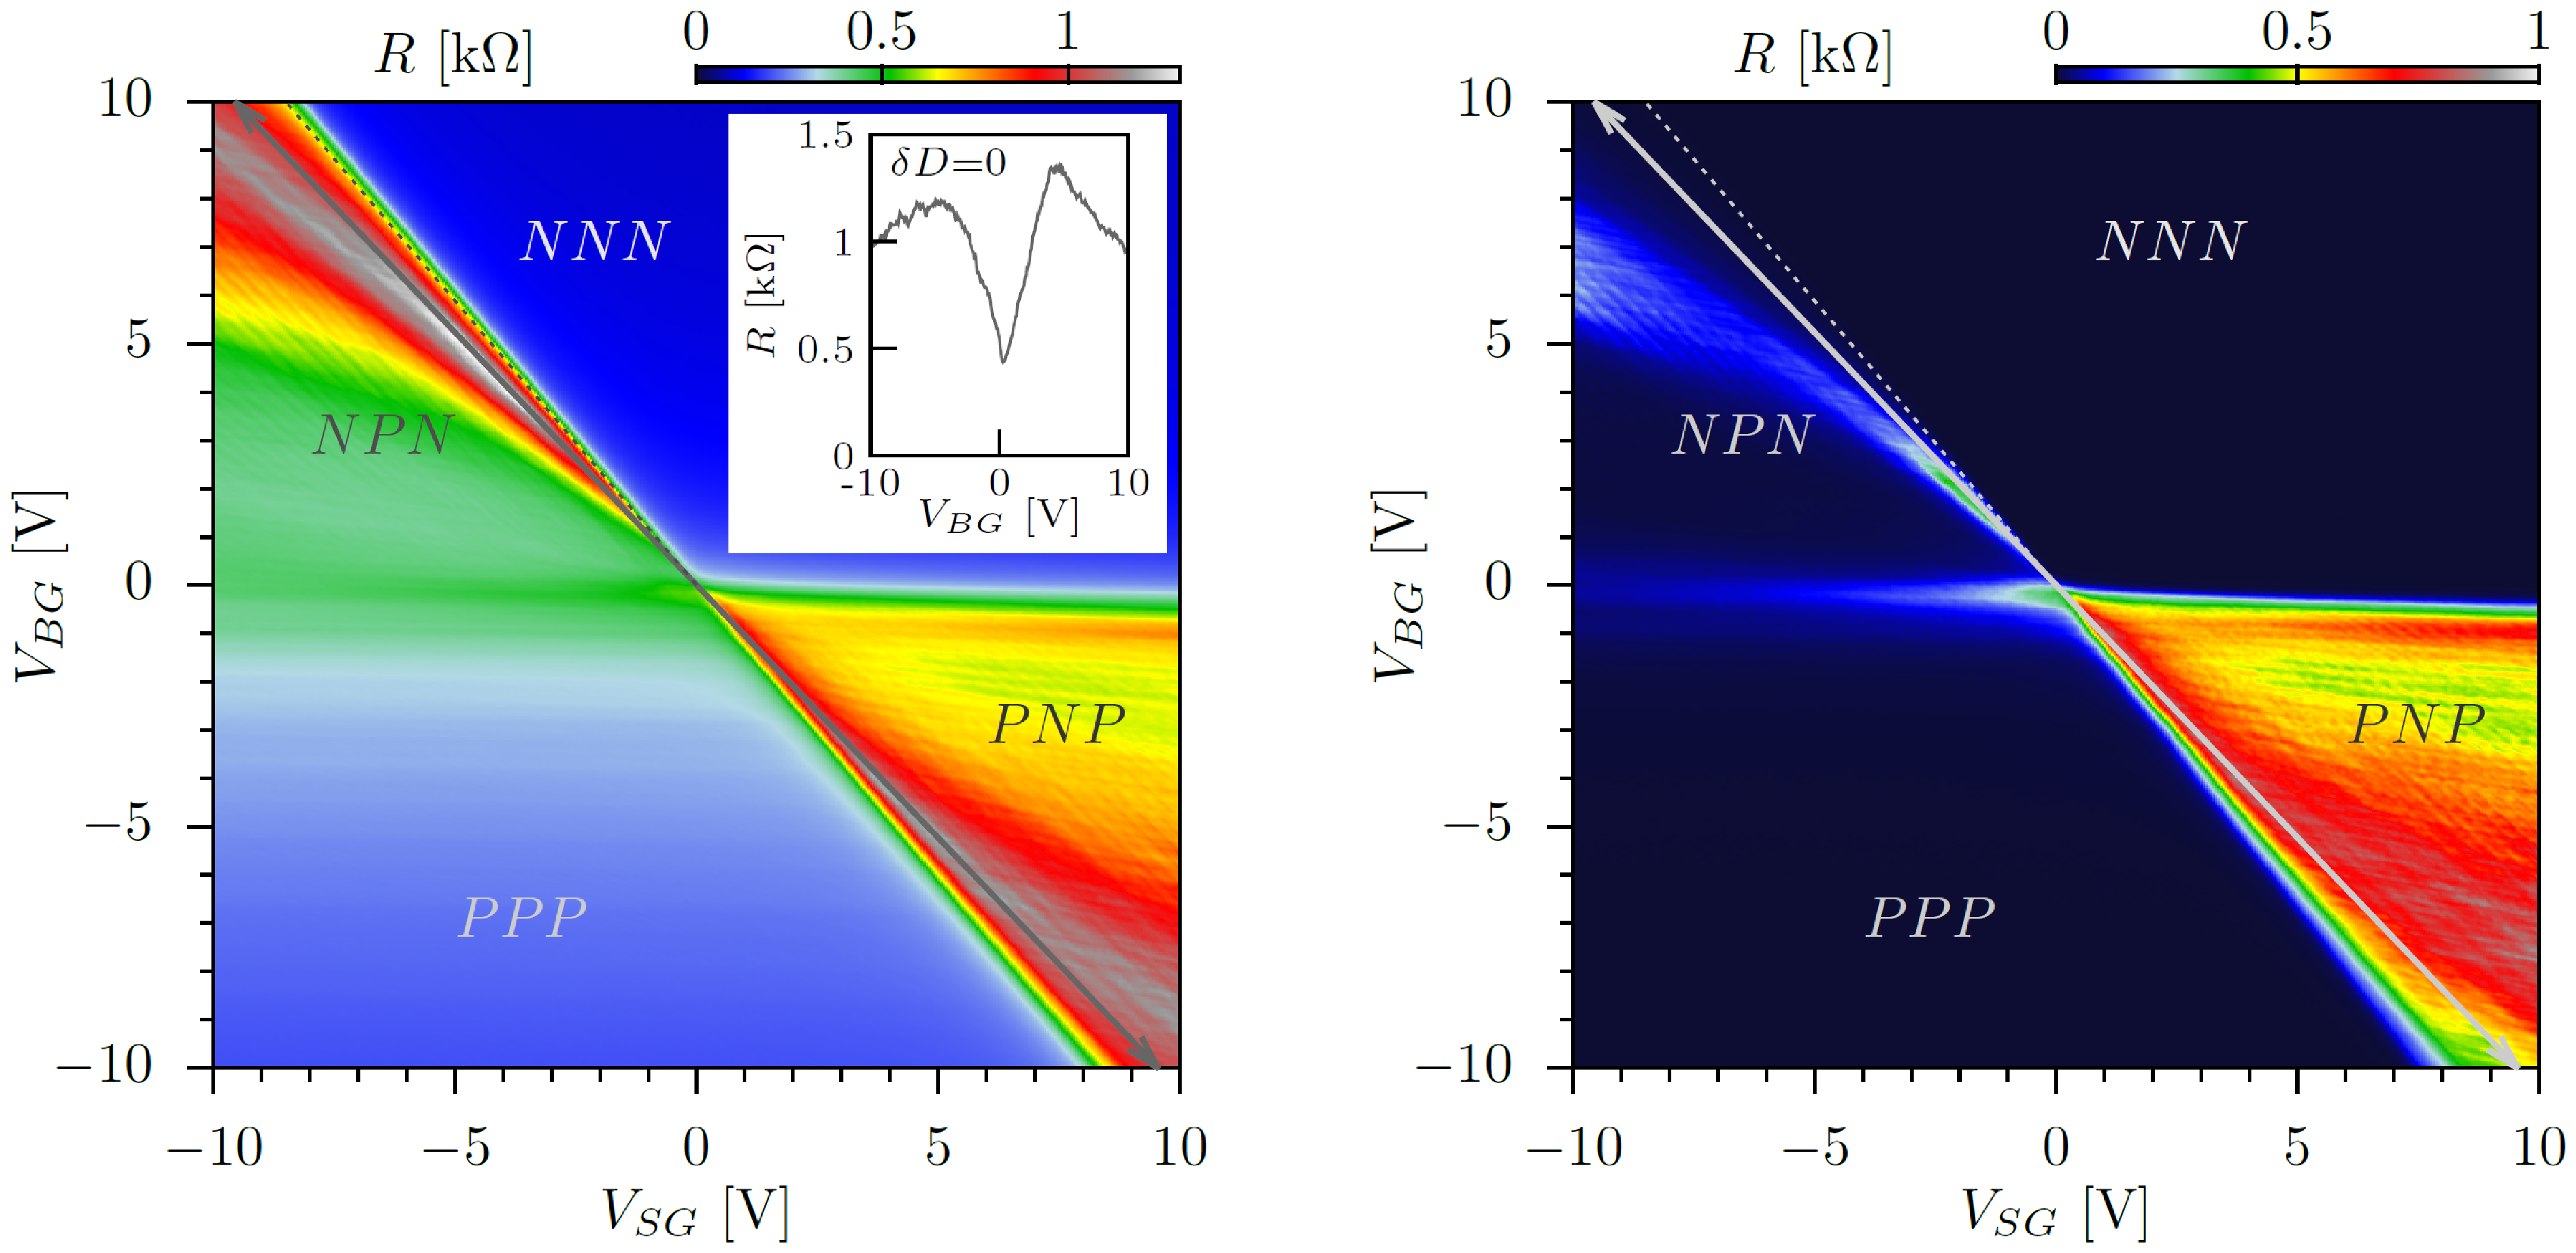
\includegraphics[width=0.8\textwidth]{figure/experiment/resistance-map-edit}
\caption{Resistance in the sample $R$ in $\text{k}\Omega$ depends on the split-gate $V_{SG}$ on the x-axis and back-gate $V_{BG}$ on the y-axis. The left picture displays data of the normal state, the right picture displays data of the superconducting state. The grey arrow indicates the displacement field line, where the fields created by back-gate and split-gate voltage are equal.}\label{fig:gate-map}
\end{figure}
In figure \ref{fig:gate-map}, the normal state resistance dependence on both back-gate and split-gate voltage is shown. The results of the normal state resistance differ from previous studies \cite{Oostinga2008}, \cite{Taychatanapat2010}. The gate map in \ref{fig:gate-map} has the back-gate as y-axis, the split-gate forming the QPC as x-axis, and the color indicates the strength of measured resistance. The diagonal line where the fields created back and split-gate are equal is called displacement field line (indicated with a grey arrow). The four quadrants are named according to how the BLG is gated: The first letter is the doping of the BLG region between the left superconductor and the split-gate, which is not gated. The middle letter indicates the doping underneath the region of the split-gate, and the third letter is the BLG doping between split-gate and right superconducting lead. Depending on the the choice of $V_{BG}$ and $V_{SG}$, the overall doping can be either one of $NNN$, $NPN$, $PPP$, or $PNP$. In the upper left quadrant, where the region is $NPN$ doped, the maximum resistance seems to follow the displament field line on the diagonal. After a certain point, however, it bends, and its maximum resistance is not found to be on the diagonal line anymore. This behaviour was not seen in  \cite{Oostinga2008}, \cite{Taychatanapat2010} -- these studies observed the maximum resistance to be on the diagonal line. The effect can be seen in the normal state resistance map, but it is strongly visible in the superconducting state. The overall resistance of the sample is higher on the p-side, because the superconducting leads are slightly n-doped. This leads to a $PN$-junction at each contact, which is seen in the gate map for the superconducting state. The $PNP$-region remains resistive, while the $NPN$-region shows zero resistance.
\begin{figure}
\centering
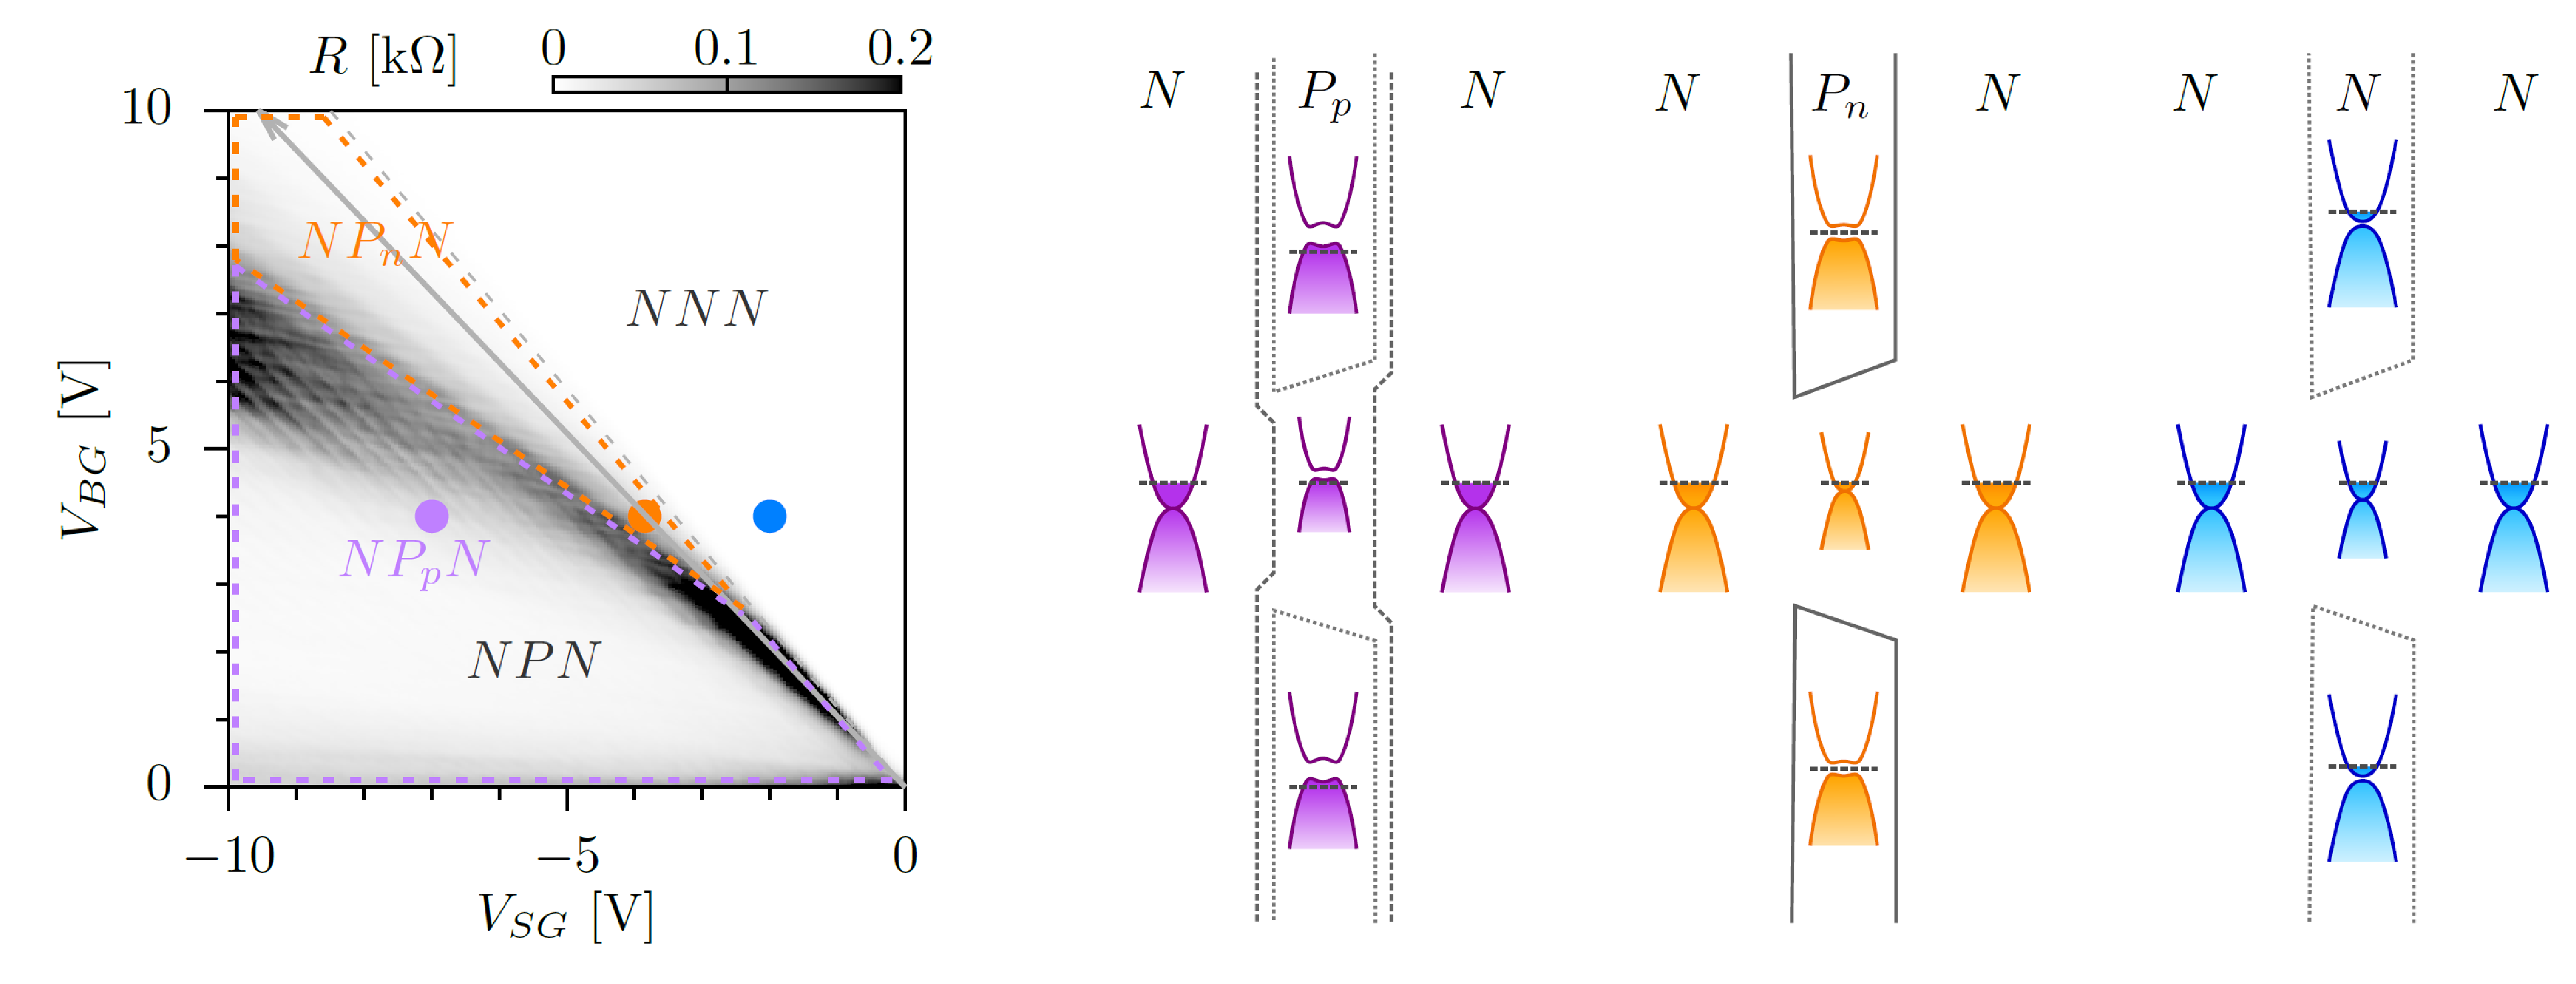
\includegraphics[width=0.5\textwidth]{figure/experiment/npn-region-detail}
\caption{A detailled view on the $NPN$-region of the resistance map. When the split-gate voltage $V_{SG}$ dominates, the area between the two split-gate fingers (the violet framed region) becomes $P$-doped because of the stray fields of the $V_{SG}$. When the constricition works as a 1D-channel, the area between the fingers (the orange framed region) is $N$-doped and the current can pass though this region. In the blue framed region, the sample is overall conductive. }\label{fig:npn-regions-gates}
\end{figure}
How can the bending in the resistance peak be explained?  Since the charge carrier density in the sample is low ($2.8\cdot 10^{18}\ \text{cm}^-2$), the influence of the back gate is important. The higher the back gate value, the less the charge carrier density is affected by the split gate and the stray fields it produces. In the lower $NPN$-region, the split gates work as intended: The channel region -- the region between the split gates where the supercurrent can pass through -- is conductive, because the back gate dominates. The BLG directly underneath the gates is $P$-doped, and the area between the two gate fingers is $N$-doped. A channel is created, where the current can pass through. This set-up is illustrated in the middle picture of figure \ref{fig:npn-regions-gates}. However, in the region where the resistance curve starts to bend, the stray fields from the split gate dominate. The area underneath the gates is still $P$-doped, but now the area between the fingers is slightly $P$-doped as well (see the right picture in figure \ref{fig:npn-regions-gates}), which effectively leads to a blocking behaviour of the channel, and eventually to an increased resistance.
%\subsection*{Fabry Perot resonances}
%gate dependece of conductance shows oscillatory behaviour, are attributed to Fabry Perot interferences of differenct cavities \cite{Shytov2008}	

\section{Superconducting State}\label{sec:experiment-superconducting}

The superconducting state is analysed in the $NPN$-region of the gatemap. The confinement of the two-dimensional supercurrent (in the case of no barrier present) to transport on a one-dimensional channel manifests in a Fraunhofer pattern of the supercurrent and in the differential conductance $dI/dV$. 
\begin{figure}
\centering
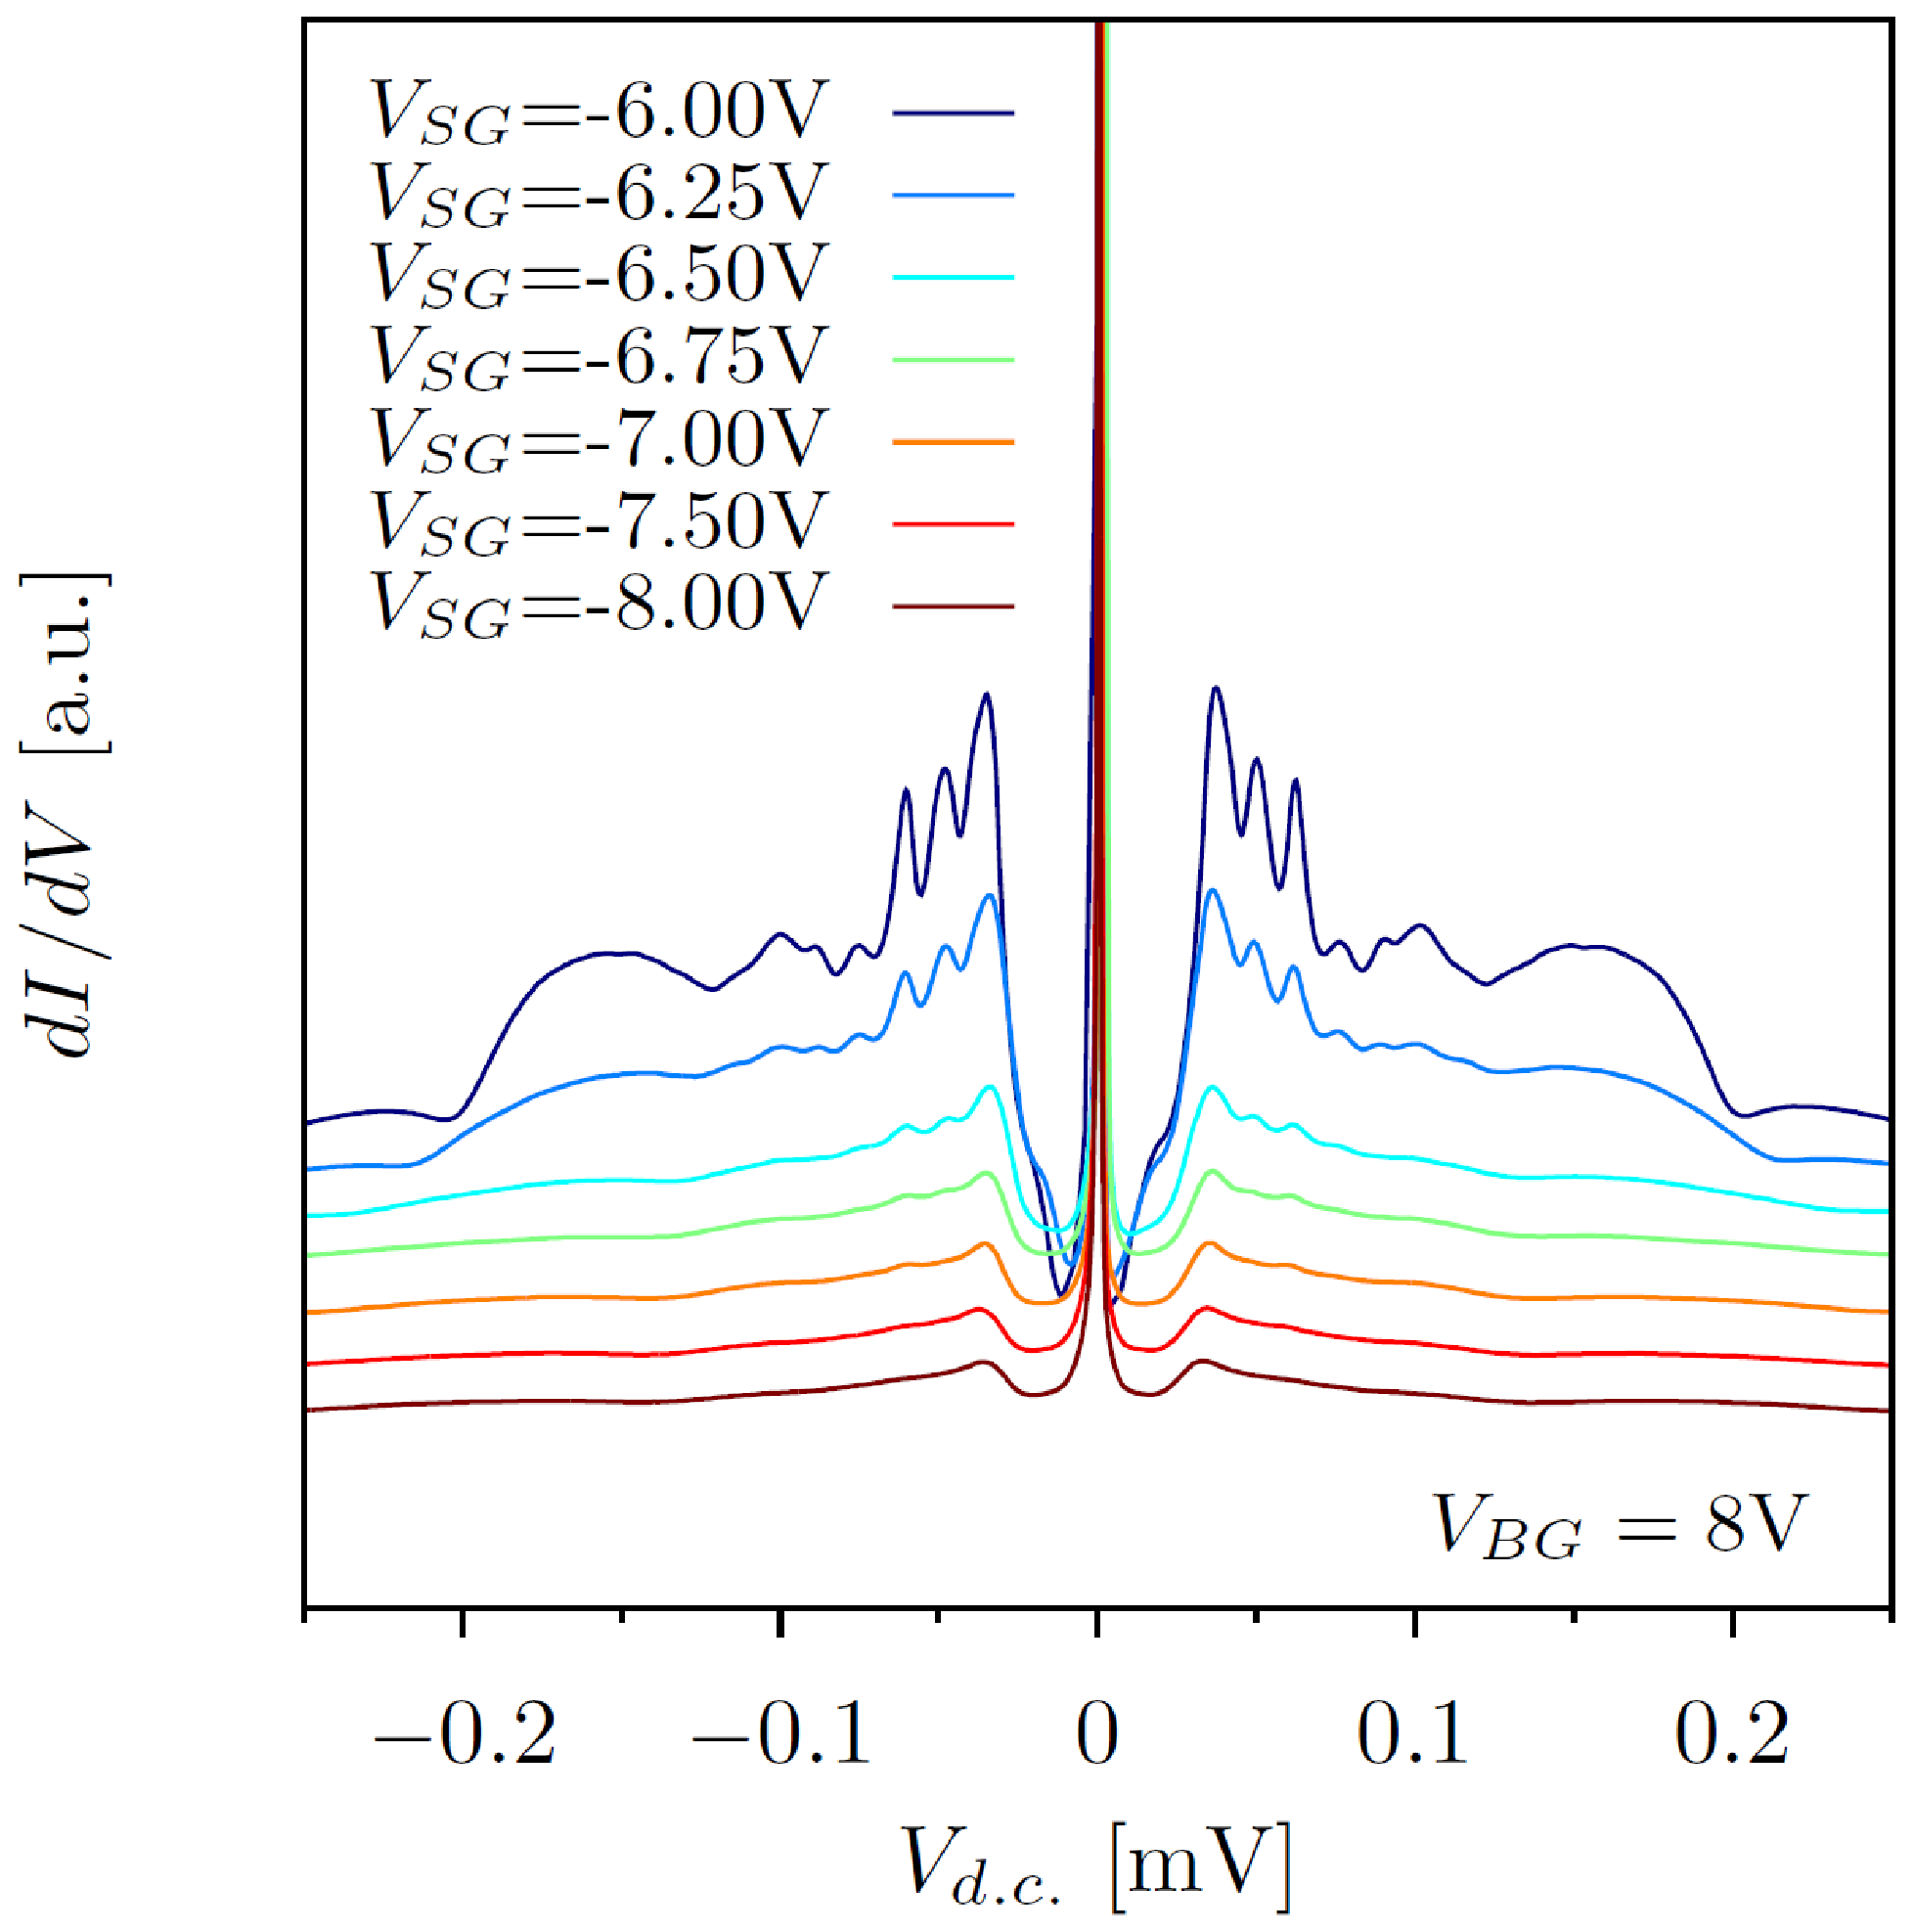
\includegraphics[width=0.4\textwidth]{figure/experiment/mar}
\caption{Differential conductance versus voltage applied for different values of $V_{SG}$. The higher the split-gate voltage, the less peaks are visible.}\label{fig:mar}
\end{figure}
While there is no constriction present, at $V_{SG} = 0 V$, multiple Andreev reflections take place. When the constriction -- the QPC barrier -- forms, the process of multiple Andreev reflections is supressed, because the probability of an electron reaching the opposite superconducting lead and getting Andreev reflected there is low. This is observable in the differential conductance for different values of the splitgate $V_{SG}$. Andreev reflection manifests within the $dI/dV$ curve in form of as peaks. In figure \ref{fig:mar}, the $dI/dV$ curves are plotted. For $V_{SG} = 0 V$ (blue curve), sharp peaks can be seen. These peaks vanish with increasing split-gate voltage.
\begin{figure}
\centering
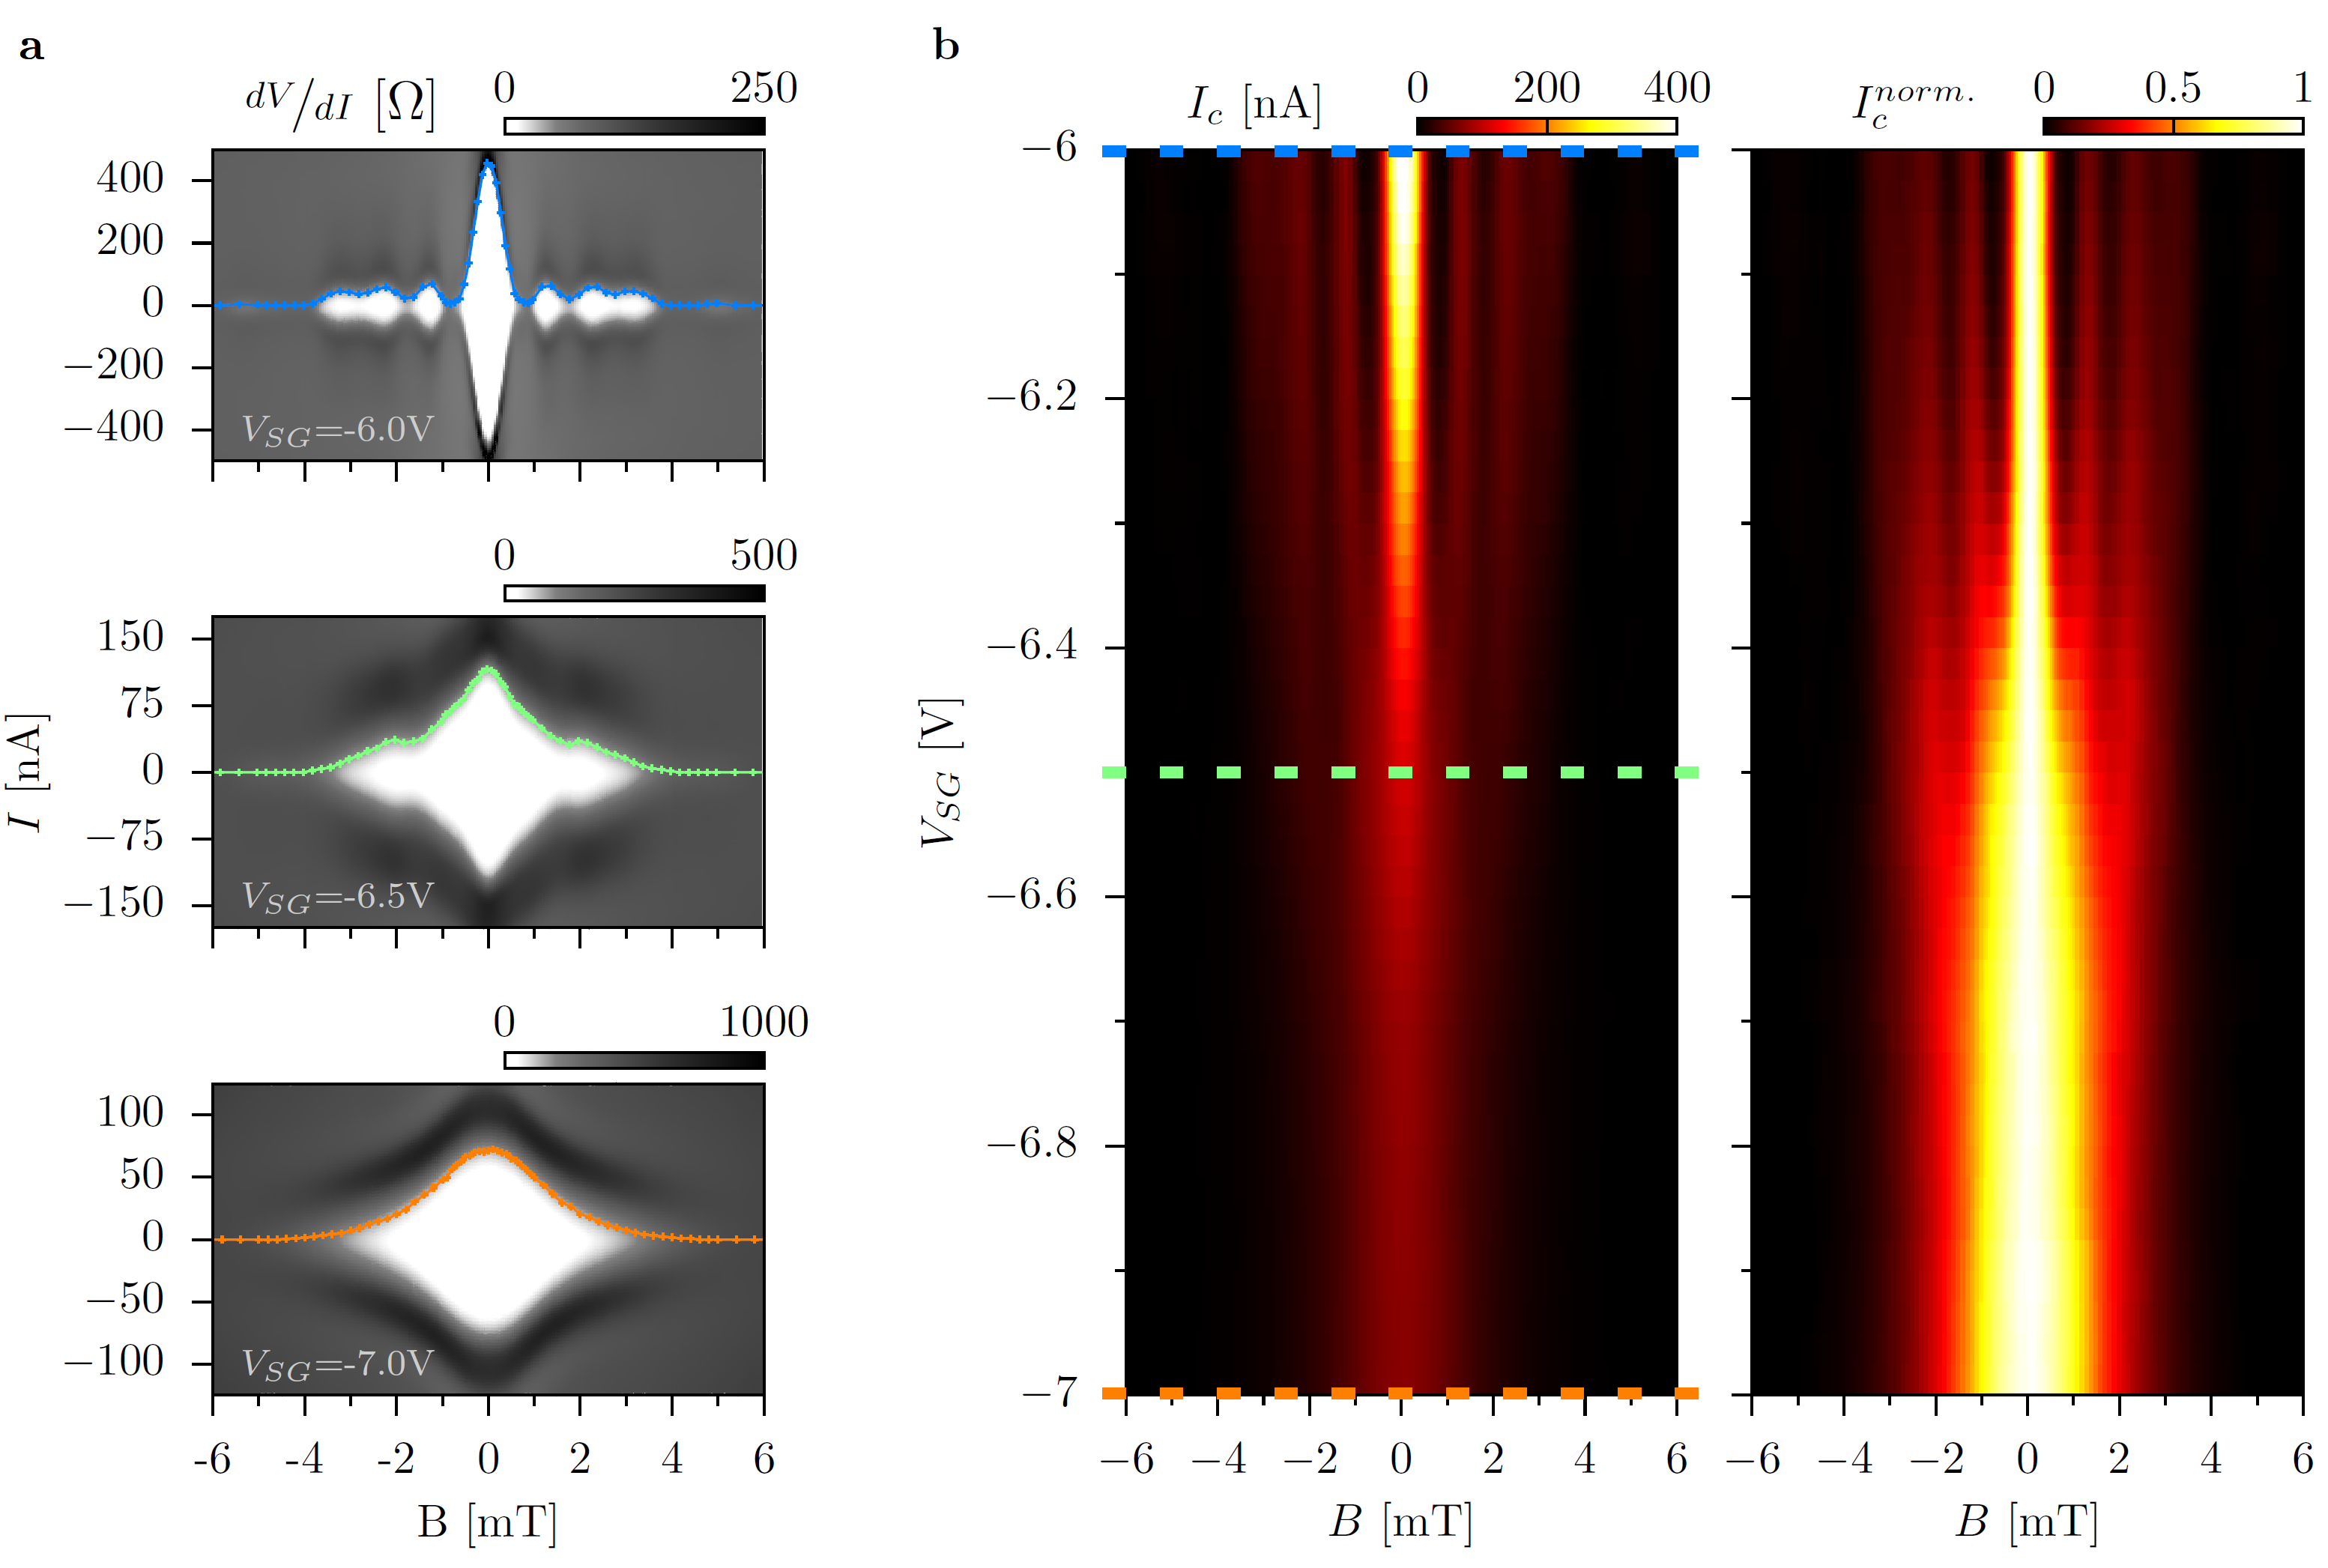
\includegraphics[width=0.8\textwidth]{figure/experiment/supercurrent}
\caption{\textbf{a} shows differential resistance $dV/dI$ plotted against the magnetic field $B$. The y-axis indicates the strength of the critical current, which is the dotted, coloured line. \textbf{b} shows the critical current (left) and normalised critical current (right) versus a magnetic field (x-axis) for different values of $V_{SG}$. The dotted curves from \textbf{a} correspond to different stadiums of the transition from 2D-Fraunhofer pattern to a bell-shaped pattern where the current is confined.}\label{fig:supercurrent}
\end{figure}
By probing the magnetic interference pattern, the supercurrent density can be explored. When the junction geometry changes, for example because the split-gate voltage is increased and a constriction starts to form, the Fraunhofer pattern will change accordingly. Figure \ref{fig:supercurrent} b) shows magnetic interferometry measurements at a constant back-gate voltage $V_{BG}$. The x-axis indicates the magnetic field $B$ and the y-axis is the split-gate voltage $V_{SG}$. The colour displays the strength of the ciritcal current. The confinement of the current can be seen in the plots in figure \ref{fig:supercurrent} a), where $I_c$ curves are plotted for $V_{SG} = -6\ V,\ -6.5\ V,\ -7\ V$. For $V_{SG} = -6 V$, the observed Fraunhofer pattern indicates a two-dimensinal current flow. With increasing $V_{SG}$, the lobes of the pattern are lifted. When the split-gate reaches $V_{SG} = -7\ V$, the constricion has formed, and the Fraunhofer pattern has vanished: A bell-shaped pattern is observed. This shows a transition from the beating to the non-beating, gaussian battern indicates that a one-dimensional channel has formed. A similar transition from a Fraunhofer pattern to a gaussian-like decay has been obeserved before, for example in \cite{Chiodi2012}, where a long SNS junction has been studied.
